\documentclass[tikz,xcolor = {svgnames, dvipsnames}, border = 2mm]{standalone}
\usepackage{tikz}
\usetikzlibrary{shapes,positioning,decorations.pathmorphing, calc, arrows}
\usepackage{amsmath}
\begin{document}
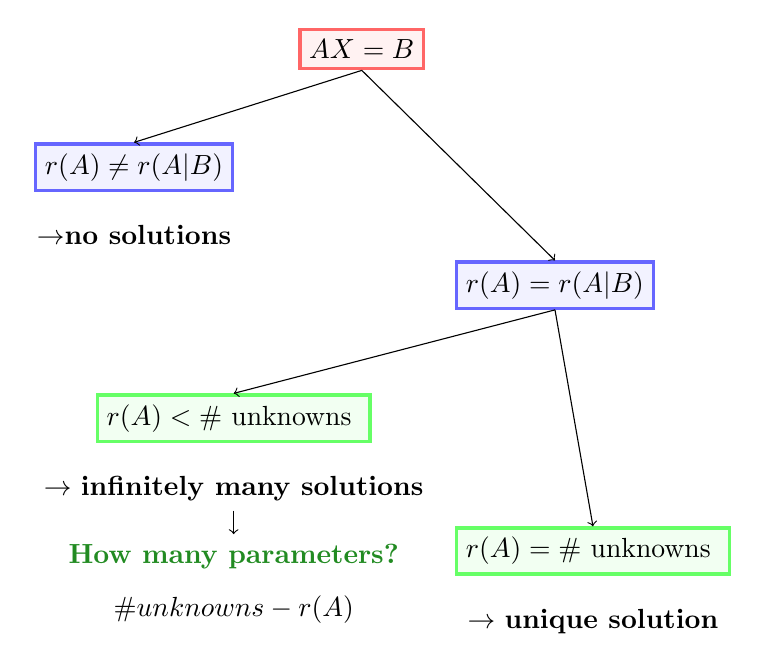
\begin{tikzpicture}[node distance = 1.5 cm, redsquare/.style={rectangle, draw=red!60, fill=red!5, very thick, minimum size=5mm}, bluesquare/.style={rectangle, draw=blue!60, fill=blue!5, very thick, minimum size=5mm}, greensquare/.style={rectangle, draw=green!60, fill=green!5, very thick, minimum size=5mm}]
\node[redsquare] (sustavi) {$AX = B$};
\node (centar) [below of = sustavi]{};
\node[bluesquare] (manji rang) [ left = of centar] {$r(A) \neq r(A|B)$};
\node (tekst 1) [below = 0.3 cm of manji rang] {$\rightarrow $\textbf{no solutions}};
\node[bluesquare] (jednak rang) [below right  = of centar] {$r(A) = r(A|B)$};
\node[greensquare] (parametri) [below left = of jednak rang] {$r(A) < \# \text{ unknowns }$};
\node (tekst) [below = 0.3 cm of parametri] {$\rightarrow$ \textbf{infinitely many solutions}};
\node  (broj) [below  = 0.3 cm of tekst] {\textcolor{ForestGreen}{\textbf{How many parameters?}}};
\node(parametri 2)[below = 0.1 cm of broj] {$\# unknowns - r(A)$};
\node[greensquare] (jedinstveno) [below right = of parametri] {$r(A) = \# \text{ unknowns }$};
\node (tekst 3) [below = 0.3 cm of jedinstveno]{$\rightarrow$ \textbf{unique solution}};

\draw[->] (sustavi.south) --(manji rang.north);
\draw[->](sustavi.south) -- (jednak rang.north);
\draw[->](jednak rang.south) -- (parametri.north);
\draw[->](jednak rang.south) -- (jedinstveno.north);
\draw[->](tekst.south) -- ( broj.north);
\end{tikzpicture}
\end{document}